
\chapter[Introdução]{Introdução}



\section[Contexto]{Contexto}

Nos últimos anos, tem surgido iniciativas isoladas de algumas entidades da Administração Pública, em procurar adotar métodos ágeis em suas equipes de desenvolvimento, com destaque para o Scrum e o \textit{Extreme Programming}-XP \cite{TCU:2013} \cite{RTMAC}.  Ainda mais recente, houve a iniciativa de mesclar o uso de métodos ágeis com a filosofia de gestão da produção, conhecida como Lean, com o foco em gerenciar o contrato dos fornecedores de desenvolvimento de \textit{software} \cite{agilebrazil}. 

\begin{comment}
Isso é um teste de comentário
\end{comment}

Lean no Desenvolvimento de \textit{Software} é uma filosofia que busca aplicar os princípios do Pensamento Lean no desenvolvimento do \textit{software}. Dentre os princípios do Lean se destacam: a eliminação de desperdícios; o respeito às pessoas envolvidas no processo; a qualidade; a simplicidade; a otimização do todo e entregas rápidas \cite{poppendieck}.

É importante ressaltar que apesar de sugerir diversas ferramentas, como o Kanban, também presente em Métodos Ágeis, o Lean está mais relacionado à forma de pensar, exige muito mais uma mudança cultural de cada organização do que a aplicação e utilização de ferramentas. 

Lean está relacionado com Métodos Ágeis, não só pela semelhança dos seus princípios e práticas, mas também porque ambos valorizam as pessoas em detrimento de ferramentas e buscam agregar valor de negócio ao sistema que está sendo desenvolvido. Do ponto de vista teórico os métodos ágeis e o Lean, se baseiam em diferentes teorias, como: teoria geral dos sistemas \cite{sistemas}, teoria da complexidade \cite{complexidade}, teoria das restrições \cite{katayama2010} e teoria de gestão da escola de relações humanas \cite{administracao}. 

Essas teorias representam um contraponto a metodologias mais prescritivas e preditivas, também conhecidas como tradicionais, que possuem seu amparo teórico principalmente na visão da teoria da administração científica, que tem como um dos percursores Frederick W. Taylor e presupõe que todo saber e tomadas de decisões são funções específicas da gerência e que os trabalhadores devem executar suas tarefas por meio de métodos e procedimentos pré-definidos \cite{administracao}.

Scrum é uma metodologia ágil desenvolvida para a gestão do processo de desenvolvimento de \textit{software}. É uma abordagem que aplica ideias de controle de processos da indústria ao desenvolvimento de \textit{software}, resultando assim, numa abordagem que reintroduz a ideia de flexibilidade, adaptabilidade e produtividade \cite{porto}. Scrum surgiu a partir do “Manifesto Ágil”, publicado em 2001, e como método ágil tem como valores: indivíduos e interações mais do que processos e ferramentas; \textit{software} funcionando para o cliente em vez de documentação; colaboração com o cliente mais do que negociação de contratos e resposta rápida às mudanças mais do que seguir planos \cite{manifesto}. 

A ideia principal é que no desenvolvimento de \textit{software} existem diversas variáveis, quer sejam de natureza ambiental ou técnica, que provavelmente mudarão ao longo da execução do processo. Essa característa torna o processo de desenvolvimento pouco previsível e complexo, requerendo flexibilidade e personalização para ser capaz de responder às mudanças. Outro sim, o contato do cliente deve ser ativo, haja visto que, ele é determinante para a criação do \textit{software}, e por consequência, afeta o próprio processo do serviço, no caso as atividades do desenvolvimento.

A terceirização de serviços em organizações públicas no contexto de contratação de empresas de desenvolvimento de \textit{software} é crescente. A gestão do processo de desenvolvimento de \textit{software} é um grande desafio para essas organizações, pois a maioria delas não são responsáveis diretamente pelo desenvolvimento do \textit{software} e ao mesmo tempo elas precisam, como contratantes, gerenciar o andamento do processo de desenvolvimento do \textit{software} de suas contratadas. 

A legislação brasileira de contratação de serviço de desenvolvimento vigente, se apoia na Lei 8.666/93, IN 04/2010 SLTI/MPOG (para Poder Executivo) e acórdãos do TCU, que serão detalhados no Capítulo 2 deste trabalho. 



\section[Justificativa]{Justificativa}

A utilização de metodologias ágeis e semelhantes em contratações de serviços de tecnologia da informação está ganhando espaço nas organizações públicas brasileiras e gerando questões importantes de estudo para a academia. Assim, recentemente, iniciativas de inserção de tais metodologias na gestão de contratos de fornecedores de desenvolvimento de \textit{software} em organizações públicas estão sendo feitas e, portanto, torna-se necessário estudos que evidenciem os resultados advindos do uso de métodos ágeis neste contexto. Uma das principais contribuições deste trabalho será evidenciar para os gestores de contratos e para os demais envolvidos no processo de gestão e desenvolvimento de \textit{software} terceirizado, os resultados do uso de métodos ágeis em contraposição aos métodos tradicionais de gestão e desenvolvimento de \textit{software}, normalmente adotados. 

\section[Problema]{Problema}

Durante muitos anos as organizações privadas e públicas utilizaram metodologias tradicionais no desenvolvimento de \textit{software} ou na gestão de contratos da terceirização do desenvolvimento das soluções de TI. Nos últimos anos, com o surgimento das metodologias ágeis, este cenário começou a mudar no contexto das instituições privadas a fim de aumentar sua produtividade, eliminar desperdícios e aumentar o valor de negócio produzido para o cliente. Nas instituições públicas essa mudança teve início recentemente. Tais organizações perceberam que uma grande quantidade de documentos estava sendo produzida e pouco \textit{software} estava sendo entregue no final do contrato \cite{TCU:2013}. Assim, a questão de pesquisa deste trabalho é:

\textit{\textbf {A utilização de métodos ágeis combinadas com o pensamento no Lean no Desenvolvimento, tornam mais eficiente o gerenciamento de contratos de terceirização de \textit{software} em organizações públicas brasileiras, ao se comparar com metodologias tradicionais?}}

\section[Objetivos]{Objetivos}

O objetivo geral deste trabalho é realizar uma investigação empírica sobre o uso da ferramenta Kanban, alinhada ao Scrum, no gerenciamento de contratos de desenvolvimento em organizações públicas, procurando evidenciar as principais dificuldades e riscos encontrados em sua adoção, bem como suas vantagens e benefícios. Dentre os objetivos específicos estão:

\begin{itemize}
\item Caracterizar o processo de contratações de soluções de TI nas organizações públicas brasileiras;
\item Caracterizar a filosofia Lean no desenvolvimento de \textit{software} e metodologias ágeis;
\item Caracterizar e relacionar o Kanban, o Lean e o Scrum;
\item Investigar aplicação de métodos ágeis e o pensamento Lean no gerenciamento de contratos de uma organização pública brasileira;
\item Definir e caracterizar um estudo de caso;
\item Coletar dados de contratos executados tanto com metodologias tradicionais quanto com metodologias ágeis, ou até mesmo sem metodologias específicas, em uma organização pública brasileira;
\item Realizar análise dos dados coletados;
\item Realizar interpretação e discursão dos resultados obtidos.
\end{itemize}

\section[Metodologia de Pesquisa]{Metodologia de Pesquisa}

Nessa seção apresenta-se a metodologia de pesquisa adotada neste trabalho.
Para isso, foram definidos: a natureza da pesquisa; o tipo de metodologia de pesquisa; o tipo de abordagem de pesquisa; os métodos de
procedimentos de pesquisa e os tipos de técnicas de coletas de dados.

Os procedimentos de pesquisa selecionados foram pesquisa bibliográfica,
documental, levantamento e estudo de caso. As técnicas de coleta de dados selecionadas foram
documentos e entrevistas. A seleção
metodológica é apresentada na Fig. (1).

	\begin{figure}[h]
		\centering
		\label{fig01}
			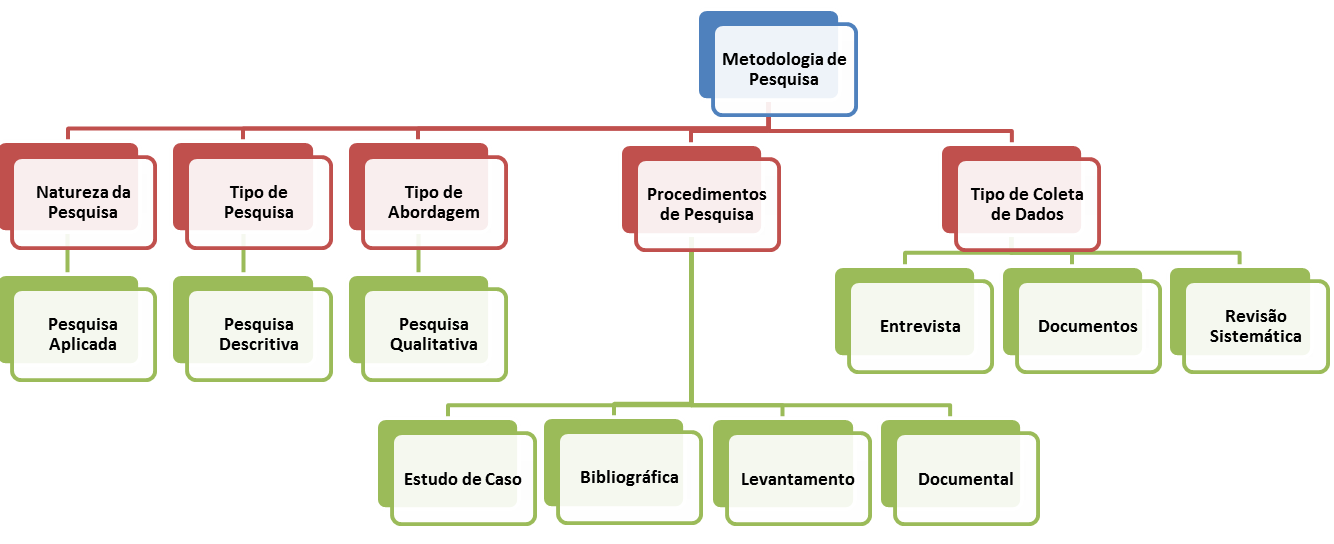
\includegraphics[scale=0.7]{figuras/metodologiapesquisa.png}
		\caption{Seleção de Metodologia de Pesquisa}
	\end{figure}

Nesta pesquisa, o esquema adotado compreende as fases: Planejamento; Coleta
de Dados; Análise e Interpretação dos dados, e Redação do Resultado. 

O Planejamento consiste na determinação da questão de pesquisa, a escolha da metodologia de pesquisa, a definicação das fases da pesquisa,  a definição dos procedimentos de pesquisa e das técnicas de coleta de dados, a construção do referencial teórico e a proposta do trabalho final.


Na Coleta de Dados são executados os procedimentos de pesquisa e as técnicas de coletas de dados a seguir:

\begin{itemize}
\item Pesquisa Bibliográfica: pesquisa realizada a partir de livros, dissertações e trabalhos relacionados à área de pesquisa;
\item Pesquisa Documental: pesquisa realizada a partir de documentos públicados por organizações públicas;
\item Estudo de Caso: utilizar um estudo de caso real de uma organização pública brasileira;
\item Entrevistas: dados serão coletados por meio de estrevistas semi-estruturadas para incremento do estudo de caso;
\item Documentos: leitura dos documentos fornecidos pelo órgão público do estudo de caso será realizada para coleta de dados para análise.
\end{itemize}

A Análise dos Resultados diz respeito a fase em que os dados coletados serão analisados e interpretados.

A Redação dos Resultados diz respeito a fase em que os resultados serão estruturados e concluídos.

\section[Organização do Trabalho]{Organização do Trabalho}

Este trabalho está organizado em cinco capítulos. Neste Capítulo 1 encontra-se a introdução do trabalho que consiste em: contexto do trabalho,  justificativa,  problema, objetivos e metodologia de pesquisa adotada.

No Capítulo 2 - Contratações de Fornecedores de Desenvolvimento de \textit{Software} - apresenta-se as principais informações referentes à Contratação de Fornecedores de Desenvolvimento de \textit{Software}. Para isso, o capítulo é iniciado com uma visão geral sobre a importância das contratações e suas principais características. Posteriormente, é apresentado um resumo das legislações relacionadas à Contratação de Soluções de Tecnologia da Informação.

No Capítulo 3 - Pensamento Lean - são apresentados os conceitos referentes ao Lean na Manufatura e ao Lean no Desenvolvimento de \textit{Software}. Com este fim, é apresentado um breve histórico sobre o surgimento do Lean na Manufatura e os seus principais princípios e práticas e, posteriormente, é apresentado como o Lean Manufatura foi adaptado para o desenvolvimento de \textit{software} e para isso é abordado os princípios e práticas do Lean no Desenvolvimento de \textit{Software}.

No Capítulo 4  - Adoção de Métodos Ágeis na Gestão de Demandas de Desenvolvimento de \textit{Software} em Organizações Públicas Brasileiras - são apresentados os princípios e valores das Metodologias Ágeis e caracterizado o Framework Scrum, posteriormente, é feito o relacionamento entre o Scrum, o Lean e o Kanban. Ainda são apresentados as iniciativas de adoção de métodos ágeis no Governo, os desafios inerentes a adoção de métodos ágeis em organizações públicas brasileiras e será caracterizado o contexto do órgão que será estudo nesse trabalho.

No Capítulo 5 - A Proposta de Trabalho - é apresentado a definição da proposta de trabalho e a definição do estudo de caso que será realizado.
